% Generated with TikZ

\documentclass[tikz,border=8pt]{standalone}
\usepackage{tikz}
\usetikzlibrary{calc,positioning,fit,backgrounds}
\usepackage{amsmath}

\tikzset{
  every picture/.append style={
    execute at end picture={
      \begin{scope}[on background layer]
        \draw[rounded corners=6pt, line width=0.8pt, gray!60]
          ([xshift=-6pt,yshift=-6pt]current bounding box.south west) rectangle
          ([xshift=6pt,yshift=6pt]current bounding box.north east);
      \end{scope}
    }
  }
}

\begin{document}
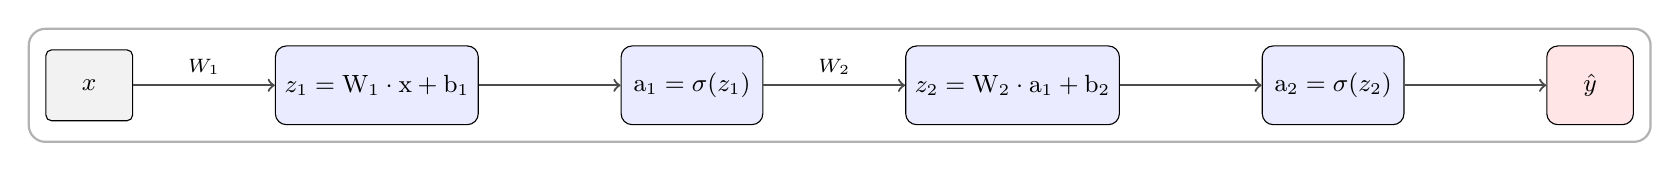
\begin{tikzpicture}[
        node distance=1.4cm,
        font=\small,
        input/.style={draw, rounded corners=2pt, minimum width=1.1cm, minimum height=0.9cm, fill=gray!10},
        hidden/.style={draw, rounded corners=4pt, minimum width=1.8cm, minimum height=1cm, fill=blue!8},
        output/.style={draw, rounded corners=4pt, minimum width=1.1cm, minimum height=1cm, fill=red!10},
        arrow/.style={->, thick, draw=black!70},
    ]

    % Input
    \node[input] (x) {$x$};

    \node[hidden, right=1.8cm of x] (weight) {$z_{1} = \mathrm{W_{1}} \cdot \mathrm{x} + \mathrm{b_{1}}$};
    \node[hidden, right=1.8cm of weight] (activation) {$\mathrm{a_1} = \sigma(z_1)$};
    \node[hidden, right=1.8cm of activation] (weight2) {$z_{2} = \mathrm{W_{2}} \cdot \mathrm{a_1} + \mathrm{b_{2}}$};
    \node[hidden, right=1.8cm of weight2] (activation2) {$\mathrm{a_2} = \sigma(z_2)$};
    \node[output, right=1.8cm of activation2] (out) {$\hat{y}$};

    % Lines
    \draw[arrow] (x) -- node[above, font=\scriptsize] {$W_1$} (weight);
    \draw[arrow] (weight) -- node[above, font=\scriptsize] {} (activation);
    \draw[arrow] (activation) -- node[above, font=\scriptsize] {$W_2$} (weight2);
    \draw[arrow] (weight2) -- node[above, font=\scriptsize] {} (activation2);
    \draw[arrow] (activation2) -- node[above, font=\scriptsize] {} (out);

\end{tikzpicture}
\end{document}
